\section{The Decode Roofline}\label{sec:roofline}
Figure~\ref{fig:roofline} is the paper's central result. It plots measured decode throughput
against model size and overlays the roofline prediction
$\tokps = \mathrm{BW}_\text{eff}/\text{bytes-per-token}$, where bytes-per-token is the quantized
model file size (every weight is read once per generated token). The measured points lie on the
prediction: decode throughput scales inversely with model bytes, and the effective bandwidth is a
large and nearly constant fraction of the platform's \SI{13.98}{GB/s} DRAM peak---\DECBWLO--\DECBWHI\%
across models. A model's byte count can shrink two ways---fewer parameters or fewer bits---and both
land on the same line: fitting all \ROOFN\ measured configurations (three parameter sizes at
Q4\_K\_M plus five quantizations of the 0.5\,B model) gives $R^2=\ROOFRALL$, and the size sweep
alone gives $R^2=\ROOFR$. A single number, model bytes, predicts decode speed regardless of whether
the bytes come from architecture or from quantization.

\begin{figure}[t]\centering
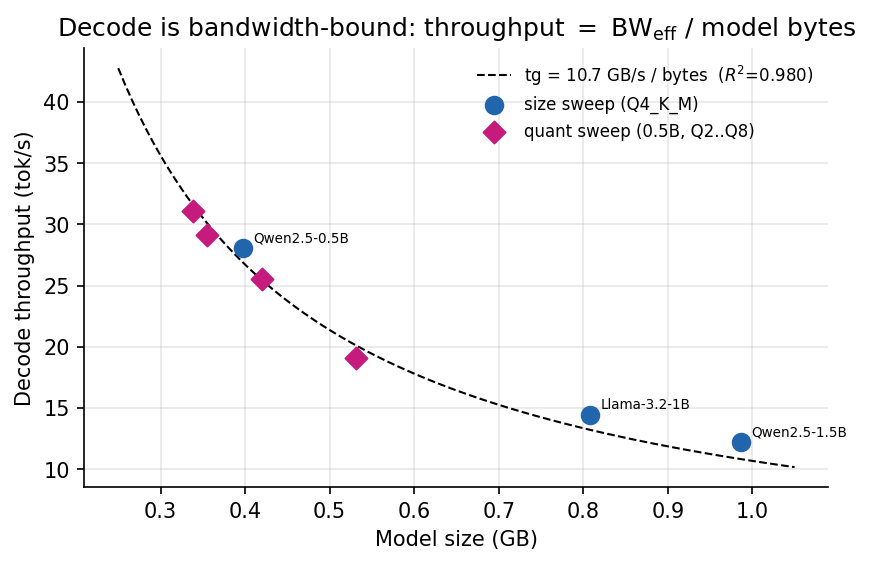
\includegraphics[width=\columnwidth]{figs/fig1_roofline.png}
\caption{Decode is bandwidth-bound. Measured decode throughput matches the roofline
$\mathrm{BW}_\text{eff}/\text{model bytes}$ (dashed) across \emph{both} the parameter-size sweep
(circles) and the quantization sweep (diamonds), sustaining \DECBWLO--\DECBWHI\% of the
\SI{13.98}{GB/s} DRAM peak ($R^2=\ROOFRALL$ over all \ROOFN\ points). Fewer bytes---from fewer
params or fewer bits---means proportionally faster decode.}
\label{fig:roofline}
\end{figure}

\textbf{Prefill vs.\ decode, and threads.} Prefill processes all prompt tokens as one
matrix--matrix product and is compute-bound: it runs \PPTGRATIO$\times$ faster than decode and
scales with thread count. Decode, a matrix--vector product per token, does not
(Fig.~\ref{fig:threads}): adding cores past the point that saturates the memory controller yields
almost nothing, exactly as for memory-bound CNNs on this platform~\cite{jacob2026memwall}. The two
phases occupy opposite ends of the roofline.

\begin{figure}[t]\centering
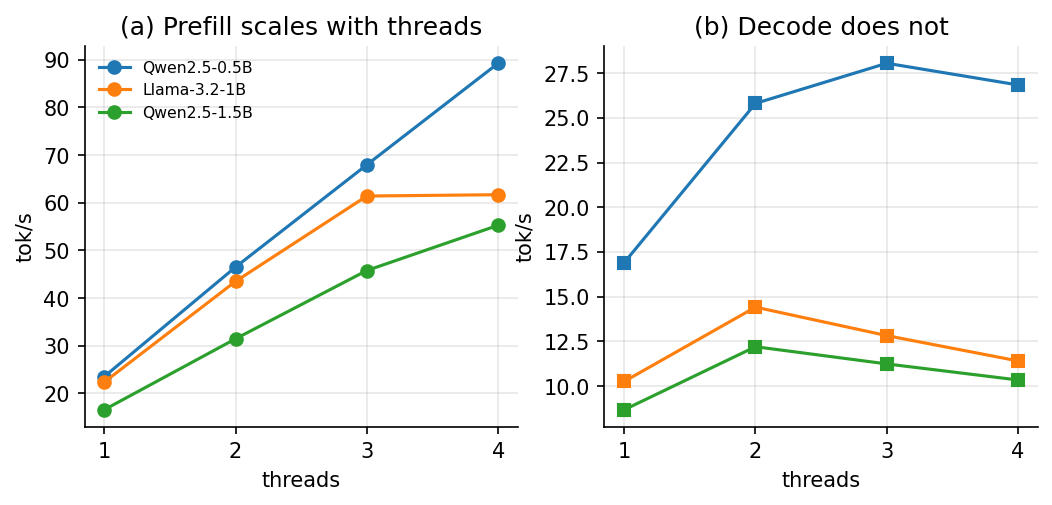
\includegraphics[width=\columnwidth]{figs/fig2_threads.png}
\caption{Thread scaling. (a) Prefill (compute-bound) scales with threads; (b) decode
(bandwidth-bound) saturates early---more cores cannot lift a memory-bound loop.}
\label{fig:threads}
\end{figure}

\section{The Quantization Frontier}\label{sec:quant}
Because decode is bandwidth-bound, reducing weight precision has a direct and predictable payoff:
fewer bytes per token means proportionally faster decode, and simultaneously a smaller footprint
that eases the capacity wall of \S\ref{sec:capacity}. Figure~\ref{fig:quant} traces
Qwen2.5-0.5B from 2 to 8 bits: decode throughput \QUANTPARA. Measured perplexity on an English
corpus completes the trade-off: \PPLPARA{} so the frontier is genuinely three-dimensional
(speed, size, quality), and on a bandwidth-bound edge device the speed and size gains from
quantization are proportional and predictable while the quality cost is the model designer's to
weigh. Quantization is thus doubly effective on a memory-constrained device---not a speed/quality
knob alone but the primary lever on throughput and memory together.

\begin{figure}[t]\centering
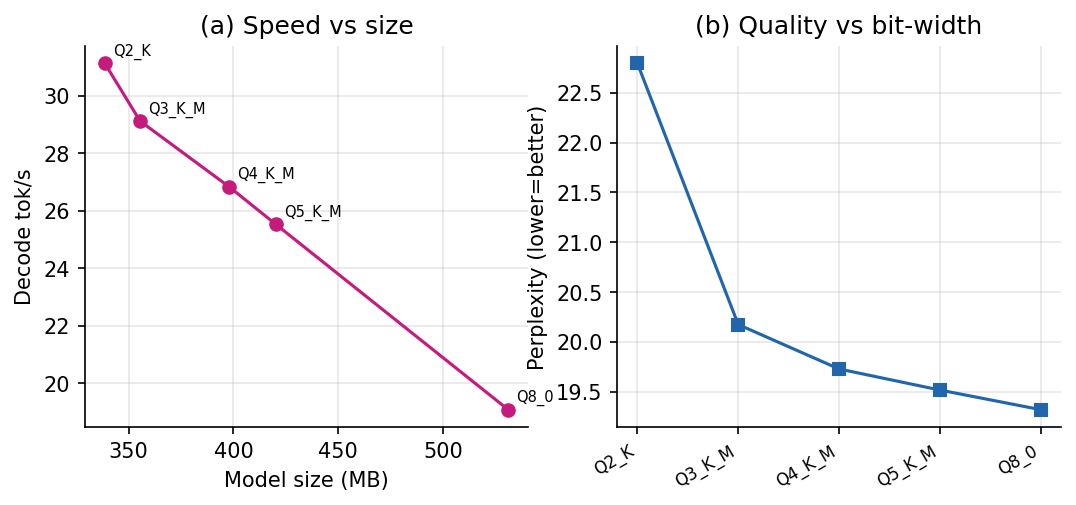
\includegraphics[width=0.85\columnwidth]{figs/fig3_quant.png}
\caption{Quantization frontier (Qwen2.5-0.5B). Lower-bit quantization moves fewer bytes per token,
raising decode throughput and shrinking the footprint together.}
\label{fig:quant}
\end{figure}

\section{The Energy of a Token}\label{sec:energy}
Figure~\ref{fig:energy} reports the PMIC-measured energy per decoded token and the DRAM-rail share
of power. \ENERGYPARA{} Strikingly, the DRAM rail contributes only \SIrange{4}{5}{\percent} of
package power: the energy cost of the memory wall is paid overwhelmingly as \emph{cores stalling}
on the VDD\_CORE rail while they wait for weights, not as DRAM-interface power. The same
counter-intuitive result held for memory-bound CNNs on this platform~\cite{jacob2026energy}; it is
the energy signature of a bandwidth-bound workload on a CPU whose cores clock far faster than its
memory can feed them.

\begin{figure}[t]\centering
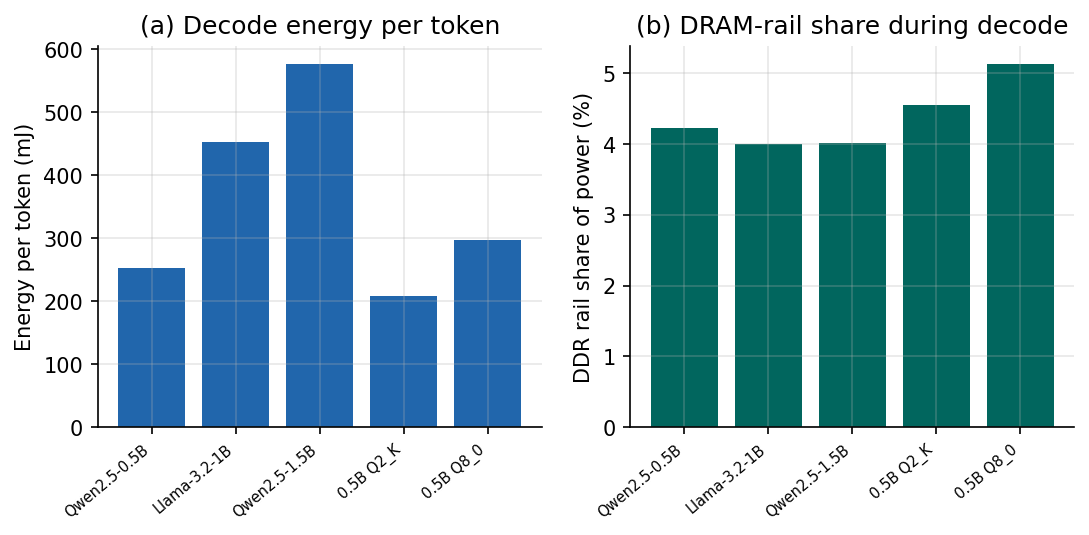
\includegraphics[width=\columnwidth]{figs/fig4_energy.png}
\caption{(a) Energy per decoded token (PMIC), rising with model size. (b) The DRAM rail is only
\SIrange{4}{5}{\percent} of package power: the memory-wall energy is paid as core stalls, not
DRAM-interface power.}
\label{fig:energy}
\end{figure}

\subsection{The Energy-Optimal Decode Clock Is Below Maximum}\label{sec:dvfs}
Since decode is bandwidth-bound, raising the CPU clock spins the cores faster while they wait on
memory: throughput barely rises but power climbs, so the energy-optimal clock is \emph{below} the
maximum (Fig.~\ref{fig:dvfs}), mirroring the memory-bound-CNN result~\cite{jacob2026energy}.
\DVFSPARA

\begin{figure}[t]\centering
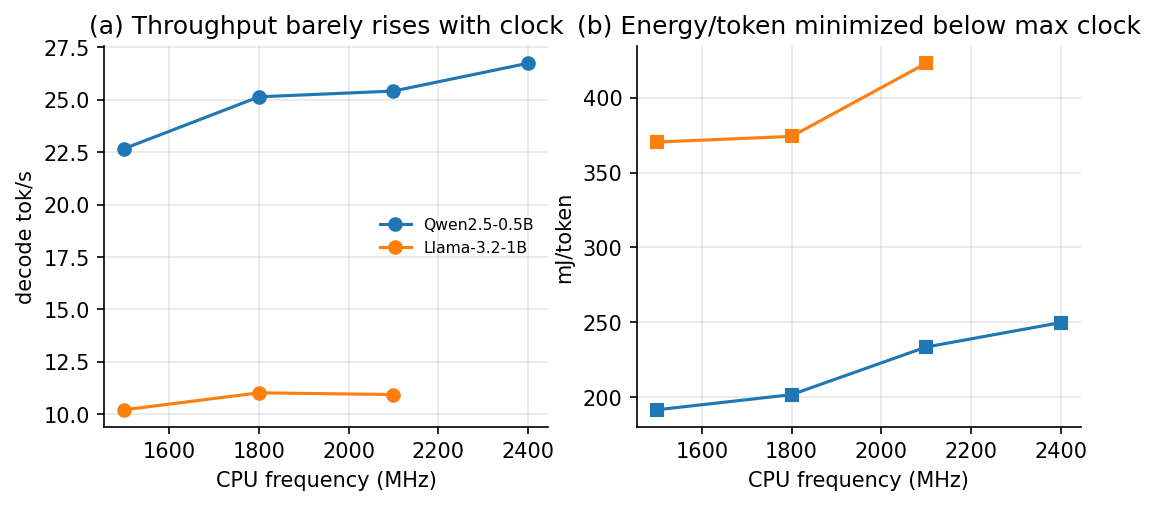
\includegraphics[width=\columnwidth]{figs/fig6_dvfs.png}
\caption{DVFS for decode. (a) Throughput is nearly flat in clock; (b) energy per token is minimized
below the maximum frequency---max-clock decode wastes energy.}
\label{fig:dvfs}
\end{figure}

\section{The KV-Cache Capacity Wall}\label{sec:capacity}
Bandwidth is one wall; capacity is the other. On 2\,GB, resident memory must hold the weights and a
KV cache that grows linearly with context length, so each model has a maximum usable context beyond
which the system swaps and decode collapses. Figure~\ref{fig:capacity} charts decode throughput
against context length; \CAPPARA{} The two walls interact: quantizing to fewer bits frees memory
for a longer context, trading precision for reach.

\begin{figure}[t]\centering
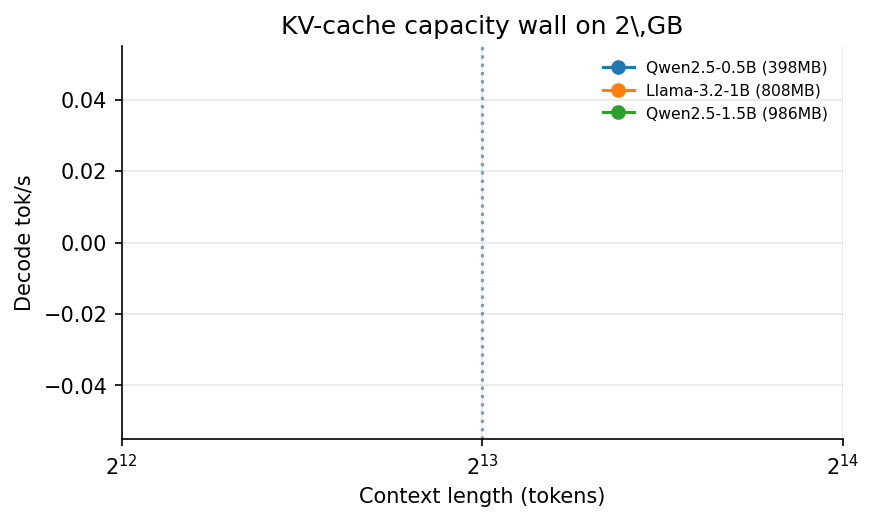
\includegraphics[width=0.9\columnwidth]{figs/fig5_capacity.png}
\caption{The KV-cache capacity wall. On 2\,GB, usable context is bounded by weights plus KV cache;
dotted lines mark where the estimated footprint exceeds the safe budget.}
\label{fig:capacity}
\end{figure}

\textbf{Weights, not KV, bound capacity at these sizes.} One might expect quantizing the KV cache
(to 8 bits) to buy substantial extra context by halving its footprint. We measured this and found
the effect is marginal for 0.5--1.5\,B models on 2\,GB: at these sizes the resident \emph{weights}
dominate the budget and the KV cache is secondary, so it is \emph{weight} quantization, not KV
quantization, that is the primary lever on capacity. KV-cache quantization would matter more for
larger models or much longer contexts, where KV grows to rival the weights---a regime the 2\,GB
device cannot reach regardless.

\section{An Energy-Optimal Configuration Policy}\label{sec:policy}
The measurements compose into a deployable policy. For a throughput target (an interactive
tokens-per-second SLO), the device should run at the \emph{lowest} clock that still meets it and
at the quantization that fits memory---because on the bandwidth-bound decode loop, additional
clock buys little throughput but costs energy. Selecting the minimum-energy frequency that meets
the SLO from the measured grid (Fig.~\ref{fig:policy}) \POLICYPARA{} The policy needs only the
per-platform constants measured here and a target rate; it is the LLM analogue of the SLA-aware
clock selection we derived for CNNs~\cite{jacob2026energy}, and it follows directly from the
memory-wall structure of decode.

\begin{figure}[t]\centering
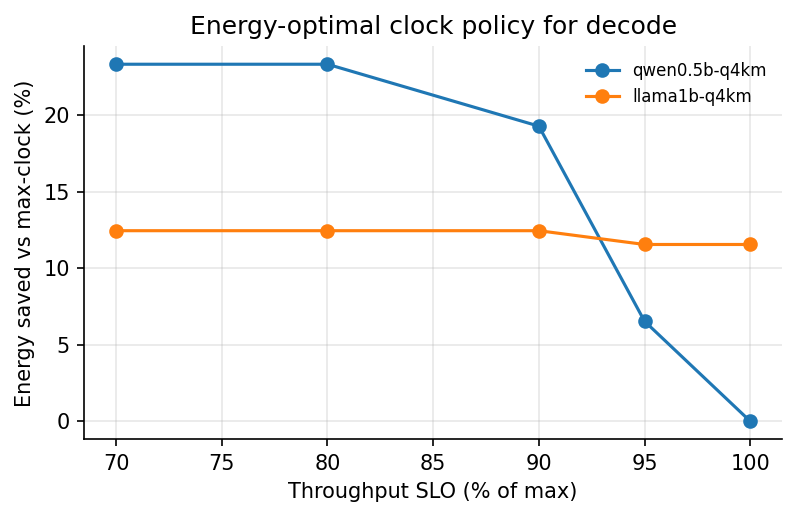
\includegraphics[width=0.85\columnwidth]{figs/fig7_policy.png}
\caption{Energy-optimal clock policy. Running the lowest clock that meets a throughput SLO saves
energy per token versus always-max-clock, at no throughput cost.}
\label{fig:policy}
\end{figure}

\section{Discussion and Limitations}\label{sec:discussion}
\textbf{Why the roofline is so predictive here.} In the datacenter, decode's low arithmetic
intensity is hidden by batching many concurrent sequences, which turns the matrix--vector product
back into a matrix--matrix product and lifts intensity above the ridge point~\cite{pope2023efficiently}.
A single-user edge device cannot batch: every token is a genuine matrix--vector product that reads
all weights once. The workload therefore sits permanently on the bandwidth-bound slope of the
roofline, which is exactly why a one-parameter model ($R^2=\ROOFR$) suffices. This is a structural
property of single-stream decode, not an artifact of our platform or runtime.

\textbf{Design implications.} (i) \emph{Report tokens-per-byte, not just tokens-per-second}: decode
throughput on a CPU edge device is set by DRAM bandwidth divided by model bytes, so a model's decode
speed is predictable from its quantized size before any run. (ii) \emph{Quantize for bandwidth, not
just memory}: on a bandwidth-bound loop, fewer bits buy proportional throughput and energy, in
addition to fitting a longer context. (iii) \emph{Do not overclock decode}: the energy-optimal
decode clock is the minimum, and the on-demand governor's default of racing to maximum wastes energy
for negligible throughput. (iv) \emph{Budget the two walls together}: bandwidth sets speed, capacity
sets reachable context, and quantization is the single knob that relaxes both.

\textbf{Threats to validity.} Our results are specific to \texttt{llama.cpp}'s CPU backend on one
Cortex-A76 platform with LPDDR4X. The absolute bandwidth and the ridge point differ across devices,
but the \emph{structure}---compute-bound prefill, bandwidth-bound decode, a size-predicted decode
roofline, a sub-maximal energy-optimal clock, and a capacity wall---follows from the arithmetic
intensity of autoregressive decode and should transfer to other CPU edge platforms; a
faster-memory or accelerator part would raise absolute throughput but leave single-stream decode
bandwidth-bound. We study models up to 1.5\,B parameters because larger models do not fit the 2\,GB
budget at usable context; the roofline extrapolates to them but we do not measure them here. The
PMIC samples at ${\sim}\SI{10}{Hz}$, so we measure throughput unperturbed and pool power over the
steady decode phase rather than integrating a single short window. Finally, we quantify throughput,
energy, and memory but not task accuracy across quantization levels; the well-documented
accuracy--bit-width trade-off~\cite{frantar2023gptq,lin2024awq} composes with, but is orthogonal to,
the bandwidth results here.
